\documentclass[11pt,reqno,final]{amsart}

\pdfcompresslevel=0
\pdfobjcompresslevel=0

\usepackage[dvipsnames]{xcolor}% adds colors
\usepackage{amsmath, amsthm}% {amsfonts, amssymb}

% New Characters
\usepackage[latin1]{inputenc}%
\usepackage[T1]{fontenc}

\usepackage{MnSymbol}
\usepackage[normalem]{ulem}% underlining

\usepackage[theoremfont, largesc]{newpxtext} % different text,math font
\usepackage{newpxmath}

\makeatletter
\DeclareMathRadical{\sqrtsign}{symbols}{112}{largesymbols}{112}
\let\sqrt=\undefined
\DeclareRobustCommand\sqrt{\@ifnextchar[\@sqrt{\mathpalette\@x@sqrt}}
\def\@x@sqrt#1#2{%
 \setbox\z@\hbox{$\m@th#1\sqrtsign{\mkern1mu #2}$}
 \mkern3mu\box\z@}
\makeatother




% Page Typesetting
\usepackage[final]{microtype}
\usepackage{relsize}
\usepackage[margin=1in]{geometry}
\usepackage{framed}
\usepackage{tikz}

\usepackage{hyperref}
\hypersetup{
  final,
  pdftitle={Math 135 - Modeling with Functions},
  pdfauthor={Bonventre}, 
  linktoc=page,
  pagebackref,
  colorlinks=true,
  citecolor=PineGreen,
  linkcolor=PineGreen,
  linkbordercolor=PineGreen,
}


% Internal References

\usepackage[inline,shortlabels]{enumitem}

\numberwithin{equation}{section} 
\numberwithin{figure}{section}

\usepackage[nameinlink,capitalise,noabbrev]{cleveref}

\crefname{equation}{}{} % get \cref to behave as \eqref

% \theoremstyle{plain} % bold name, italic text
\newtheorem{theorem}[equation]{Theorem}%
\newtheorem*{theorem*}{Theorem}%
\newtheorem{lemma}[equation]{Lemma}%
\newtheorem{proposition}[equation]{Proposition}%
\newtheorem{corollary}[equation]{Corollary}%
\newtheorem{conjecture}[equation]{Conjecture}%
\newtheorem*{conjecture*}{Conjecture}%
\newtheorem{claim}[equation]{Claim}%
\newtheorem{question}{Question}

\theoremstyle{definition} % bold name, plain text
\newtheorem{definition}[equation]{Definition}%
\newtheorem*{definition*}{Definition}%
\newtheorem{example}[equation]{Example}%
\newtheorem*{example*}{Example}%
\newtheorem{remark}[equation]{Remark}%
\newtheorem{notation}[equation]{Notation}%
\newtheorem{convention}[equation]{Convention}%
\newtheorem{assumption}[equation]{Assumption}%
\newtheorem{exercise}[question]{Exercise}

% ---------- macros
\newcommand{\set}[1]{\left\{#1\right\}}%
\newcommand{\sets}[2]{\left\{ #1 \;|\; #2\right\}}%
\newcommand{\longto}{\longrightarrow}%
\newcommand{\into}{\hookrightarrow}%
\newcommand{\onto}{\twoheadrightarrow}%

\usepackage{harpoon}
\newcommand{\vect}[1]{\text{\overrightharp{\ensuremath{#1}}}}

\newcommand{\del}{\partial}%

\newcommand{\ki}{\chi}
\newcommand{\ksi}{\xi}
\newcommand{\Ksi}{\Xi}

% %%%%%%%%%%%%%%%%%%%%%%%%%%%%%%%%%%%%%%%%%%%%%%%%%%%%%%%%%%%%%%%%%%%%%%%%%%%%%%%%%%%%%%%%%%%%%%%%%%%%

\begin{document}

\begin{center}
        \textbf{\Large Math 135, Calculus 1, Fall 2020}\\[10pt]
        {\large 09-09: Functions, Trig, and Domains (Sections 1.3--1.4)}
\end{center}

\thispagestyle{empty}

\renewcommand{\thesection}{\Alph{section}}

\section{Meet your classmates}

Share and discuss ``how to make toast'':
\begin{question}
        Spend 3-5 minutes individually writing or drawing instructions for how to make toast.
        Once everyone in your group is ready, take turns sharing and explaining your steps.

        What were some common elements? What were some differences in your recipes?
\end{question}

\section{Angles, the Unit Circle, and Trigonometry}

We measure angles using the \textbf{unit circle}, a circle of radius 1 centered at the origin.
An angle of \textbf{1 radian} is equal to the angle made by 1 unit of arc length along the unit circle.
The circumference of the unit circle is $2 \pi$ units, so there are $2 \pi$ radians in a circle.

To convert between radians and degrees, we use the formula
\[
        180^\circ = \pi \mbox{ rad}
\]

\begin{minipage}{.48\textwidth}
        \begin{framed}
                The functions ``cosine'' $\cos(\theta) $ and ``sine'' $\cos(\theta)$
                are defined to by the $x$-coordinate and $y$-coordinate the point on the unit circle at an angle of $\theta$ \textbf{radians}.
        \end{framed}
\end{minipage}
\begin{minipage}{.48\textwidth}
        \begin{center}
                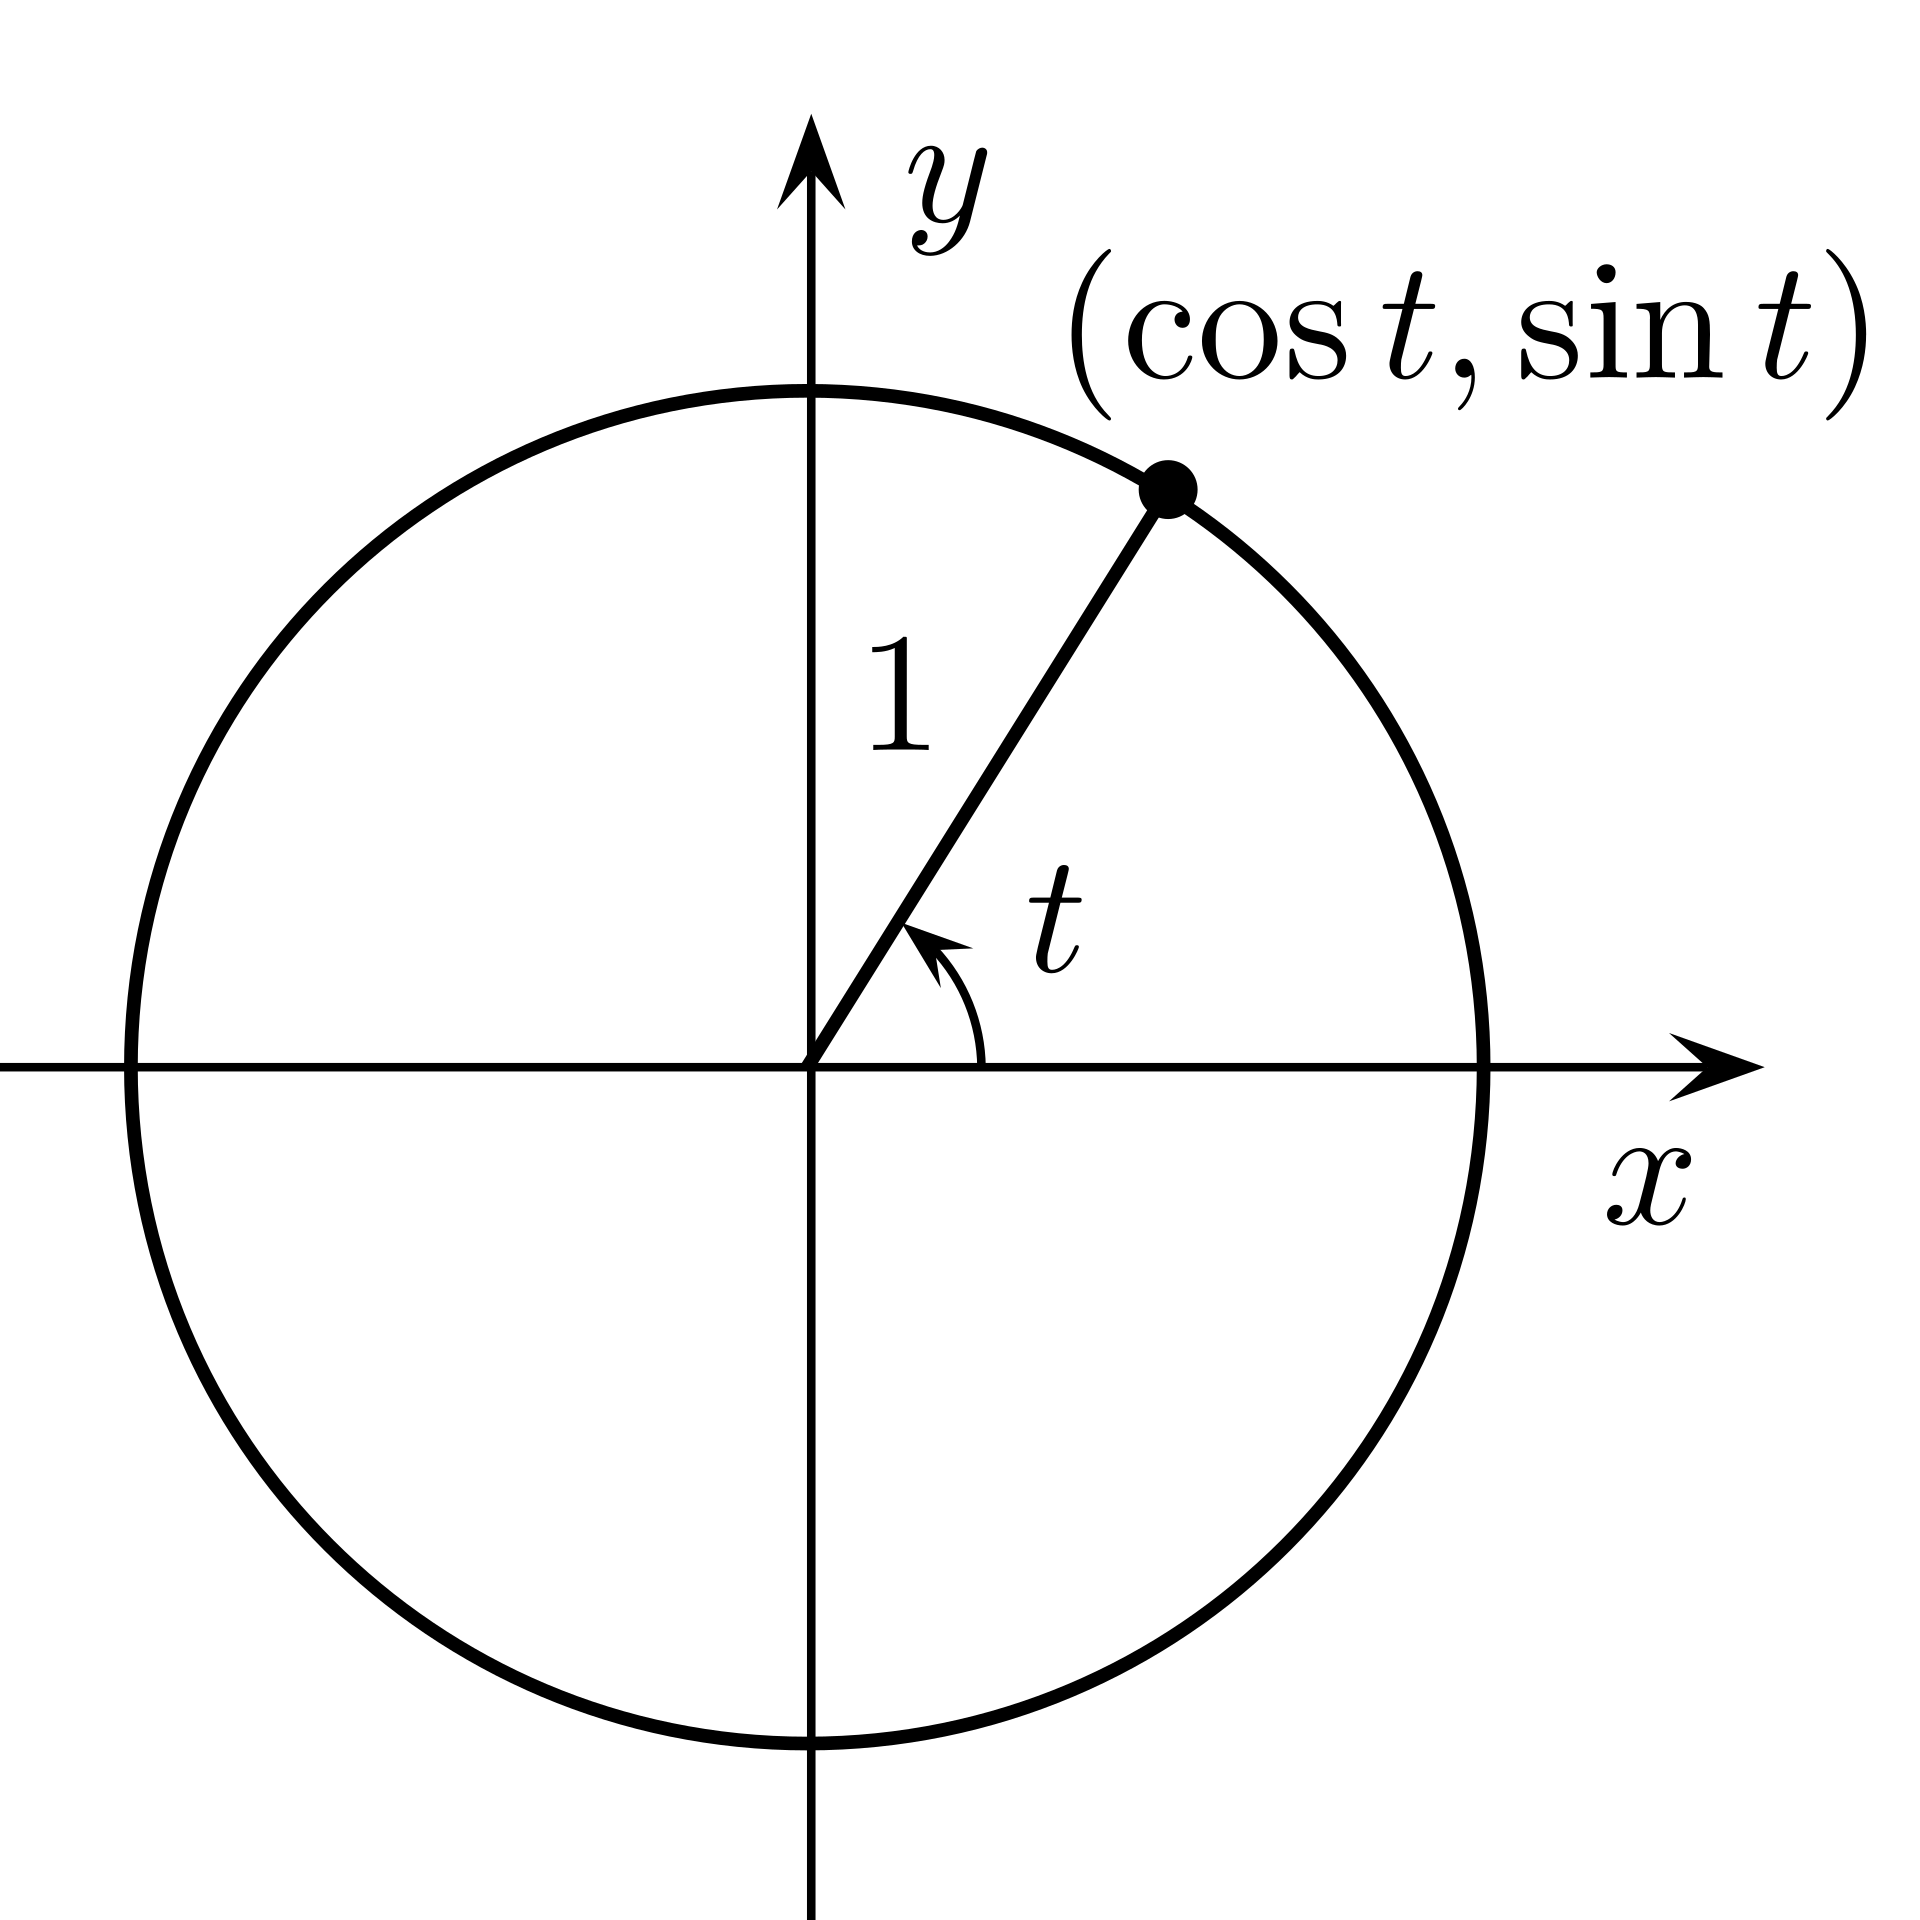
\includegraphics[width=1.8in]{09-09P_sincos.png}
        \end{center}
\end{minipage}


\begin{exercise}
        Without using a calculator, compute:\\[10pt]
        \begin{enumerate*}[(i)]
        \item $135^{\circ}$ in radians \qquad \qquad
        \item $7\pi/6$ rad in degrees \qquad \qquad 
        \item $\cos(3\pi/2)$ \qquad \qquad \qquad
        \item $\sin(45\pi)$ \qquad \qquad 
        \end{enumerate*}
\end{exercise}

$ $\\

By the Pythagorean Theorem, we have the \textbf{fundamental relationship}
        \begin{framed}
                \[
                        \cos^2(\theta) + \sin^2(\theta) = 1 \quad \mbox{for any angle $\theta$}
                \]
        \end{framed}

\subsection*{Other Trig Functions}

$ $

\begin{framed}
        \[
                \tan \theta = \dfrac{\sin \theta}{\cos \theta}
                \qquad
                \cot \theta = \dfrac{\cos \theta}{\sin \theta}
                \qquad
                \sec \theta = \dfrac{1}{\cos \theta}
                \qquad
                \csc \theta = \dfrac{1}{\sin \theta}
        \]
\end{framed}

\begin{exercise}
        Use the fundamental identity to derive the equation
        \[
                \tan^2(\theta) + 1 = \sec^{2}(\theta).
        \]
        \vfill
\end{exercise}

\newpage

\begin{minipage}{.5\textwidth}
\begin{center}
        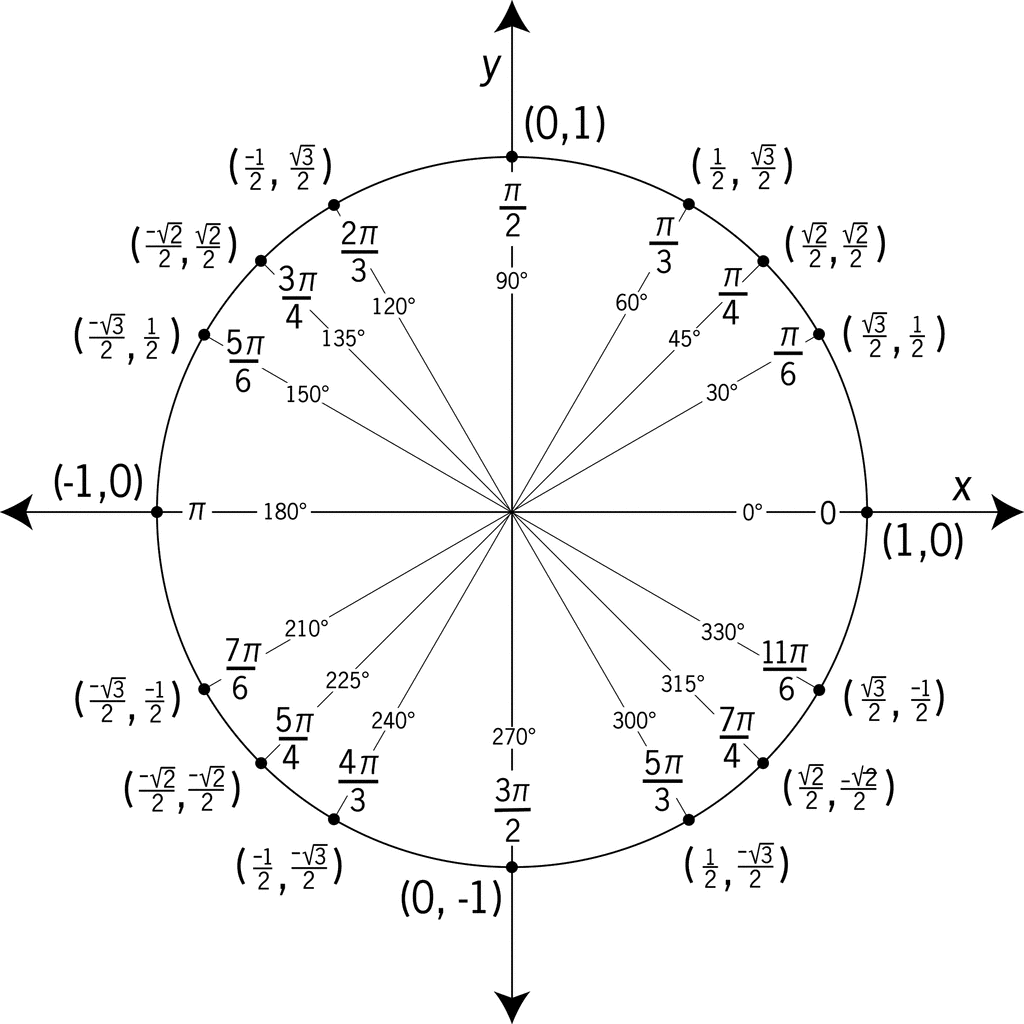
\includegraphics[width=3in]{09-09P_unitcircle.png}
        \qquad
\end{center}
\end{minipage}
\begin{minipage}{.5\textwidth}
        \begin{exercise}
                Complete the following table:
                {\renewcommand{\arraystretch}{3}%                
                  \begin{center}
                          \begin{tabular}{c|c|c|c}
                            function & \quad domain \quad $ $& \quad range \quad $ $ & even/odd?\\ \hline
                            $\cos \theta$ &&& \\
                            $\sin \theta$ &&& \\
                            $\tan \theta$ &&& \\ 
                          \end{tabular}
                  \end{center}
                }
        \end{exercise}
\end{minipage}

\begin{exercise}
        Suppose $\sin \theta = \dfrac{3}{5}$, and that $\frac{\pi}{2} < \theta < \pi$.
        Find the values of $\cos \theta$, $\tan \theta$, and $\csc \theta$.\\
        (Hint: \textbf{SOH-CAH-TOA})
        \vfill
\end{exercise}

\begin{exercise}
        Find all solutions to the equations below, assuming that $0 \leq \theta \leq 2 \pi$.\\
        \begin{enumerate*}[(a)]
        \item $\sin \theta = \dfrac{-1}{2}$ \qquad \qquad $ $ \qquad \qquad $ $ \qquad \qquad $ $
        \item $\tan \theta = \sqrt{4}$
        \end{enumerate*}
        \vfill
\end{exercise}

\newpage

\section{Other Classes of Functions}



\begin{framed}
        Other types of functions we will consider in this class include:\\
        \begin{itemize}
        \item \textbf{polynomial:} $f(x) = a_n x^n + a_{n-1}x^{n-1} + \dots + a_1 x + a_0$\\ 
        \item \textbf{rational:} $f(x) = \dfrac{p(x)}{q(x)}$, \quad where $p(x)$ and $q(x)$ are polynomials\\
        \item \textbf{algebraic:} any combination of \textit{addition, multiplication, division, and powers (e.g. $\sqrt{x}$, $x^{3/2}$)}\\
        \item \textbf{exponential:} $f(x) = C \cdot b^{tx}$
        \end{itemize}        
\end{framed}

\begin{question}
        What are two things that can go wrong to make the domain of a function smaller than ``all real numbers''?\\[10pt]
\end{question}


\begin{exercise}
        Complete the following table:\\
        \begin{center}
                {
                  \renewcommand{\arraystretch}{1.5}%                
                  \begin{tabular}{c||c|c|c|c}
                    function & \qquad type \qquad $ $ & \qquad domain \qquad $ $& \qquad range \qquad $ $ & even/odd?\\ \hline\hline
                             &&&& \\
                    $f(x) = 3x+4$ &&&& \\
                             &&&& \\ \hline
                             &&&& \\
                    $f(x) = 4x^2+1$ &&&& \\
                             &&&& \\ \hline
                             &&&& \\
                    $f(x) = \dfrac{4x^2+1}{3x+4}$ &&& $\bigtimes$ & \\
                             &&&& \\\hline
                             &&&& \\
                    $f(x) = 7\sqrt{x-1}$ &&&& \\
                             &&&& \\ \hline
                             &&&& \\
                    $f(x) = 3 \cdot \left(\frac{1}{2}\right)^{\pi x}$ &&&& \\
                             &&&& 
                  \end{tabular}
                }
        \end{center}
\end{exercise}


\end{document}

